\documentclass[14pt,a4paper,UTF8,twoside]{article}

\usepackage{amsmath}
\usepackage{graphicx}
\usepackage{geometry} 
\usepackage{ctex}
\usepackage{booktabs} % 表格库
\usepackage{titlesec} % 标题库
\usepackage{fancyhdr} % 页眉页脚库
\usepackage{lastpage} % 页码数库
\usepackage{listings} % 代码块包
\usepackage{xcolor}
\usepackage[hidelinks]{hyperref}
\usepackage{tikz}
\usepackage{tikz-qtree}
\usepackage{float} % 浮动体环境
\usepackage{subfigure} % 子图排版(多图时用)

%———————————————插入多图—————————————————%

% \begin{figure}[htbp]
%     \centering
%     \subfigure[Fig1] {
%     \includegraphics[scale=0.25]{Fig1.png} \label{1}
%     }
%     \quad
%     \subfigure[Fig2] {
%     \includegraphics[scale=0.25]{Fig2.png} \label{2} 
%     }
%     \caption{Results of Experiment}
% \end{figure}

%———————————————定义颜色—————————————————%

\definecolor{mygreen}{rgb}{0,0.6,0}
\definecolor{mygray}{rgb}{0.5,0.5,0.5}
\definecolor{mymauve}{rgb}{0.58,0,0.82}

\date{} % 留空,以让编译时去除日期

%———————————————注意事项—————————————————%

% 1、如果编译显示失败,但没有错误信息,就是 filename.pdf 正在被占用
% 2、在文件夹中的终端使用 Windows > xelatex filename.tex 也可编译

%—————————————华东师范大学———————————————%

% 论文制作时须加页眉,页眉从中文摘要开始至论文末
% 偶数页码内容为:华东师范大学硕士学位论文,奇数页码内容为学位论文题目

%————————定义 \section 的标题样式————————%

% 注意:\chapter 等命令,内部使用的是 \thispagestyle{plain} 的排版格式
% 若需要自己加上页眉 实际是在用 \thispagestyle{fancy} 的排版格式
% 加上下面这一段指令,就能够让 \section 也使用 fancy 的排版格式
% 本质就是让目录、第一页也能够显示页眉、页脚

\fancypagestyle{plain}{
  \pagestyle{fancy}
}

\title{华东师范大学软件学院实验报告} % 模板
\titleformat{\section}
    {\normalfont\bfseries\Large} % 字体大小、字体系列(\bfseries 为加粗)
    {\thesection}{1em}{}


% 设置章节的中文格式
\renewcommand\thesection{\chinese{section} \hspace{0pt}}
\renewcommand\thesubsection{\arabic{subsection} \hspace{0pt}}
% \renewcommand\thesubsubsection{\alph{subsubsection} \hspace{0pt}} % 字母编号
    

%—————————————页面基础设置———————————————%

\geometry{left=10mm, right=10mm, top=20mm, bottom=20mm}

%————————————设置页眉、页脚——————————————%

\pagestyle{fancy} % 设置 plain style 的属性

% 设置页眉

\fancyhead[RE]{\leftmark} % Right Even 偶数页右侧显示章名 \leftmark 最高级别章名
\fancyhead[LO]{\rightmark} % Left Odd 奇数页左侧显示节名 \rightmark 第二级别节名
\fancyhead[C]{华东师范大学软件学院实验报告} % Center 居中显示
\fancyhead[LE,RO]{~\thepage~} % 在偶数页的左侧,奇数页的右侧显示页码
\renewcommand{\headrulewidth}{1.2pt} % 页眉与正文之间的水平线粗细

% 设置页脚:在每页的右下脚以斜体显示书名

\fancyfoot[RO,RE]{\it Lab Report By \LaTeX} % 使用意大利斜体显示
\renewcommand{\footrulewidth}{0.5pt} % 页脚水平线宽度

% 设置页码:在底部居中显示页码

\pagestyle{fancy}
\fancyfoot[C]{\kaishu 第 \thepage 页 \ 共 \pageref{LastPage} 页} % LastPage 需要二次编译以获取总页数

%——————————————代码块设置———————————————%

\lstset {
    backgroundcolor=\color{white},   % choose the background color; you must add \usepackage{color} or \usepackage{xcolor}
    basicstyle=\footnotesize,        % the size of the fonts that are used for the code
    breakatwhitespace=false,         % sets if automatic breaks should only happen at whitespace
    breaklines=true,                 % sets automatic line breaking
    captionpos=bl,                   % sets the caption-position to bottom
    commentstyle=\color{mygreen},    % comment style
    deletekeywords={...},            % if you want to delete keywords from the given language
    escapeinside={\%*}{*},          % if you want to add LaTeX within your code
    extendedchars=true,              % lets you use non-ASCII characters; for 8-bits encodings only, does not work with UTF-8
    frame=single,                    % adds a frame around the code
    keepspaces=true,                 % keeps spaces in text, useful for keeping indentation of code (possibly needs columns=flexible)
    keywordstyle=\color{blue},       % keyword style
    % language=Python,               % the language of the code
    morekeywords={*,...},            % if you want to add more keywords to the set
    numbers=left,                    % where to put the line-numbers; possible values are (none, left, right)
    numbersep=5pt,                   % how far the line-numbers are from the code
    numberstyle=\tiny\color{mygray}, % the style that is used for the line-numbers
    rulecolor=\color{black},         % if not set, the frame-color may be changed on line-breaks within not-black text (e.g. comments (green here))
    showspaces=false,                % show spaces everywhere adding particular underscores; it overrides 'showstringspaces'
    showstringspaces=false,          % underline spaces within strings only
    showtabs=false,                  % show tabs within strings adding particular underscores
    stepnumber=1,                    % the step between two line-numbers. If it's 1, each line will be numbered
    stringstyle=\color{orange},      % string literal style
    tabsize=4,                       % sets default tabsize to 2 spaces
    % title=Python Code              % show the filename of files included with \lstinputlisting; also try caption instead of title
}

% 注释掉的部分用于后续插入代码,参数可调整,格式如下:

% 1、直接插入
% \begin{lstlisting}[language = ? , title = { ? } ]
%       Your code here.
% \end{lstlisting}
% 注意,Title 不能有下划线,否则会报错。

% 2、文件插入
% \lstinputlisting[language = C , title = ?.c] {filename.c}

%———————————————字体设置————————————————%

% \setCJKmainfont{SimSun} % 设置正文罗马族的 CJK 字体
% \renewcommand{\normalsize}{\fontsize{12pt}{15pt}\selectfont} % 设置正文字号
\linespread{1.2}

%———————————————超链接设置——————————————%

\hypersetup{
    pdfstartview=FitH, % 设置PDF文档打开时的初始视图为页面宽度适应窗口宽度(即页面水平适应)
    CJKbookmarks=true, % 用对CJK(中文、日文、韩文)字符的书签支持,确保这些字符在书签中正确显示
    bookmarksnumbered=true, % 书签带有章节编号。这对有章节编号的文档很有用
    bookmarksopen=true, % 文档打开时,书签树是展开的,方便查看所有书签
    colorlinks, % 启用彩色链接。这样,链接在PDF中会显示为彩色,而不是默认的方框
    pdfborder=001, % 设置PDF文档中链接的边框样式。001 表示链接周围没有边框,仅在单击时显示一个矩形
    linkcolor=blue, % 设置文档内部链接(如目录中的章节链接)的颜色为蓝色
    anchorcolor=blue, % 设置锚点链接(即目标在同一文档内的链接)的颜色为蓝色
    citecolor=blue, % 设置引用(如文献引用)的颜色为蓝色
}

%——————————————导言区结束,进入正文部分———————————————%

%——————————————————————————————————————%

\begin{document}

\maketitle

\begin{center} % \extracolsep{\fill} 拉伸到页面最大宽度前,保证居中显示

    \begin{tabular*}{\textwidth}{@{\extracolsep{\fill}} l  l  l }
        \hline
        实验课程:计算机系统 &  年级:2023级本科  &  实验成绩: \\
        实验名称:$ Lab5 - Malloc \ Lab $ & 姓名:张梓卫 \\
        实验编号:(5) & 学号:10235101526 & 实验日期:2024/06/03 \\
        指导老师:肖波 & 组号: \\
        \hline
    \end{tabular*}

\end{center}

\tableofcontents % 目录也需要二次编译

\section{实验简介}
\subsection{实验目的}
本实验是$CSAPP$的$Malloc\ Lab$,目的是通过实现一个动态内存分配器,加深对内存分配和管理的理解。

\subsection{实验前置准备}

\subsection{实验要求}
\begin{itemize}
    \item 不允许在 $mm.c$ 程序中定义任何全局或静态复合数据结构,例如数组、结构、树或列表等规则。
    \item 在本实验中,我们将为C程序编写一个动态存储分配器($malloc$、$free$和$realloc$例程,
    实现一个正确,高效和快速的分配器。
    \item 本实验性能指标有两个方面,内存利用率和吞吐量,我们定义的分配器需要平衡这两个指标,以获取更高的分数。
    \item 我们需要完善以下函数:
    \begin{lstlisting}[language = C , title = { Function List } ]
    int mm_init(void);
    void *mm_malloc(size_t size);
    void mm_free(void *ptr);
    void *mm_realloc(void *ptr, size_t size);
    \end{lstlisting}
    \item 实验工具:$mdriver$工具,可以检测正确性和性能。
\end{itemize}






\section{Part A 实验内容}
\subsection{堆栈分配}
堆的地址是连续的,一整块内存区域都是堆,那么如何管理这一整块内存区域呢。有三种常见的方式
\begin{itemize}
\item 隐式空闲列表(Implicit Free List):

把整块堆切分为许多紧邻的块,每个块的头部包含了这个块的大小以及它是否被分配的信息,通过这个块的大小我们就能找到与它相连的下一块的起始地址。
    \begin{itemize}
        \item 好处:简单
        \item 坏处:每次申请时需要从头开始遍历,吞吐量低下,且容易产生许多空间碎片
    \end{itemize}

\item 显式空闲列表(Explicit Free Lists):

对隐式空闲列表的改进,在隐式空闲列表基础上,每个空闲块除了存储它的大小和是否被分配的信息外,还存储了指向下一个和/或上一个空闲块的指针,这样查找空闲块的时候只需要遍历空闲列表
    \begin{itemize}
        \item 好处:提高了内存分配效率,降低空间碎片
        \item 坏处:需要多的空间存储指针,维护困难
    \end{itemize}

\item 分离空闲列表(Segregated Free Lists):

维护多个空闲链表,每个链表中的块有大致相等的大小,分配器维护着一个空闲链表数组
    \begin{itemize}
        \item 好处:更加提高了内存分配效率,降低空间碎片
        \item 坏处:维护困难,可能导致空间利用率不高
    \end{itemize}

我们的目的:平衡好吞吐率和空间利用率(这两个其实是冲突的,不可能吞吐率高又空间利用率高,因为高的吞吐率必然采用诸如链表,哈希表,树等结构,这些结构必然导致空间利用率降低,所以得平衡)
\end{itemize}

\href{https://blog.csdn.net/m0_65591847/article/details/132922447}{原文链接:堆栈分配}

堆栈相关的知识如下所示,我们要做的就是用以上的方法实现一个动态内存分配器,加深对内存分配和管理的理解。

\begin{figure} [H]
    \centering
    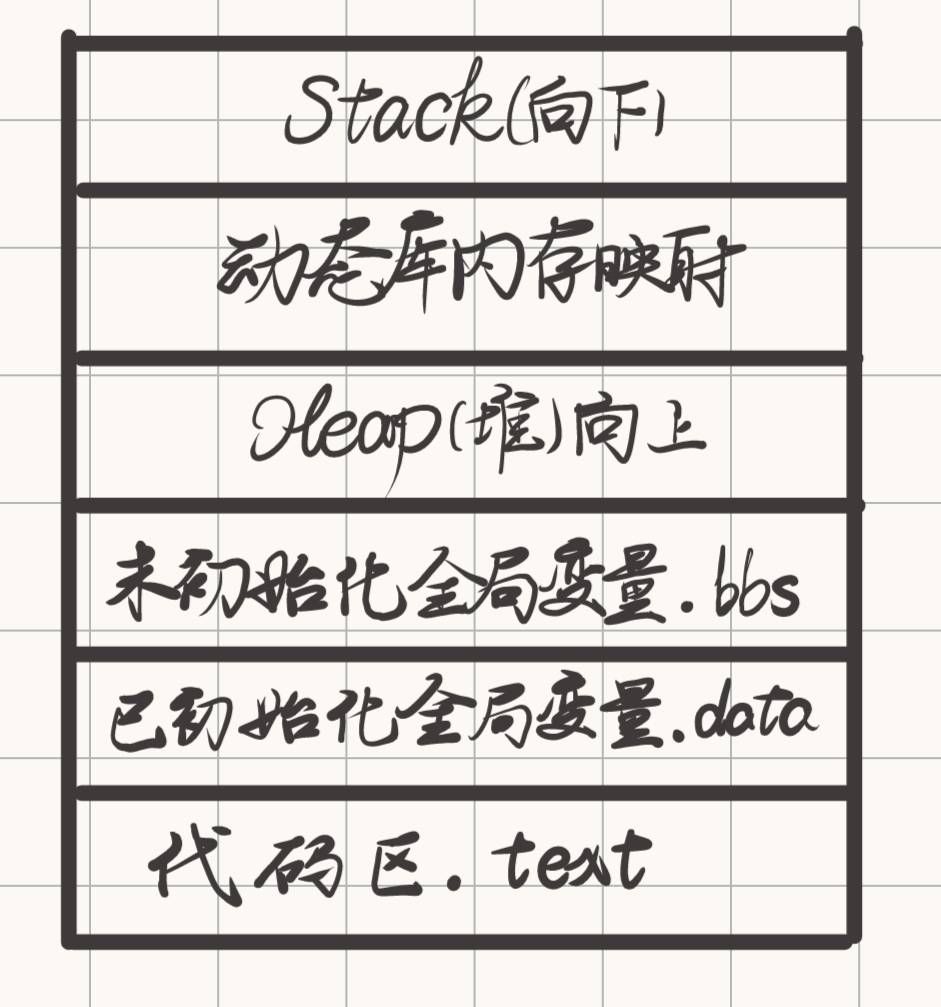
\includegraphics[width=0.42\textwidth]{Stack.jpg}
    \caption{堆栈分配} 
\end{figure}

查找空闲块的三个方法:
\begin{itemize}
    \item 1.首次适配:选择第一个合适的块。
    \item 2.下次适配:每次搜索从上次结束的地方开始。
    \item 3.最佳适配:选择大小合适的最小块。
\end{itemize}

\subsection{代码分析及填充}
对于速度($thru$)而言,我们需要关注$malloc$、$free$、$realloc$每次操作的复杂度。

对于内存利用率($util$)而言,我们需要关注$Internal \ Fragmentation$ (块内损失)和 $External \ Fragmentation$ (块是分散不连续的,无法整体利用)。

即我们$Free$和$Malloc$的时候要注意整体大块利用(例如合并$free$块、$realloc$的时候判断下一个块是否空闲)。

按照老师的要求,我首先选择实现双字对齐,隐式链表,采用首次适配。

按照$mm.c$中的内容补充一些宏定义以及函数定义,如下所示:

\begin{lstlisting}[language = C , title = { Define List } ]
    /* Basic constants and macros */

    #define WSIZE 4 // Word and header/footer size (bytes)
    #define DSIZE 8 // Double word size (bytes)
    #define CHUNKSIZE (1<<12) // Extend heap by this amount (bytes)

    #define MAX(x,y) ((x)>(y)?(x):(y)) // Maximum of two values

    #define PACK(size,alloc) ((size)|(alloc)) // Pack a size and allocated bit into a word

    #define GET(p)     (*(unsigned int *)(p)) // Read a word at address p
    #define PUT(p,val) (*(unsigned int *)(p) = (val)) // Write a word at address p
    #define GET_SIZE(p)  (GET(p) & ~0x7) // Read the size and allocated fields from address p
    #define GET_ALLOC(p) (GET(p) & 0x1) // Read the allocated field from address p

    // Given block ptr bp, compute address of its header and footer
    #define HDRP(bp) ((char *)(bp) - WSIZE)
    #define FTRP(bp) ((char *)(bp) + GET_SIZE(HDRP(bp)) - DSIZE)

    // Given block ptr bp, compute address of next and previous blocks
    #define NEXT_BLKP(bp) ((char *)(bp) + GET_SIZE(((char *)(bp) - WSIZE)))
    #define PREV_BLKP(bp) ((char *)(bp) - GET_SIZE(((char *)(bp) - DSIZE)))

\end{lstlisting}

接下来是需要定义的函数和辅助函数:

\begin{lstlisting}[language = C , title = { Function List } ]
    /* 内部编程的函数原型 */
    extern void *extend_heap(size_t words); // 扩展堆
    extern void *coalesce(void *bp); // 合并空闲块
    extern void *find_fit(size_t size); // 查找合适的空闲块
    extern void place(void *bp,size_t asize); // 分配空闲块
    extern int mm_init (void); // 初始化
    extern void *mm_malloc (size_t size); // 分配
    extern void mm_free (void *ptr); // 释放
    extern void *mm_realloc(void *ptr, size_t size); // 重新分配
    static char *heap_listp = 0; //指向块首的指针
\end{lstlisting}

接下来,我们对函数进行填充:

\begin{figure} [H]
    \centering
    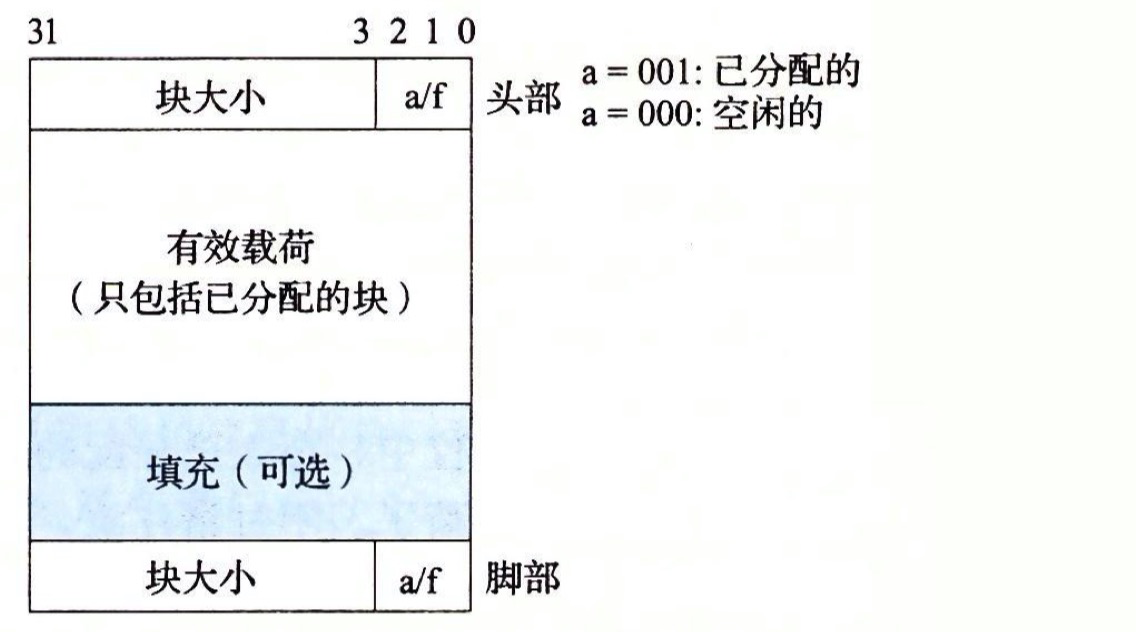
\includegraphics[width=0.42\textwidth]{BlockSize.png}
    \caption{块大小解释}
\end{figure}

\begin{lstlisting}[language = C , title = { mm\_init.c } ]
    int mm_init(void) 
    {
        /* Create the initial empty heap */
        if ((heap_listp = mem_sbrk(4*WSIZE)) == (void *)-1) // 申请4个字节
            return -1;
        PUT(heap_listp, 0);                          // Alignment padding
        PUT(heap_listp + (1*WSIZE), PACK(DSIZE, 1)); // Prologue header
        PUT(heap_listp + (2*WSIZE), PACK(DSIZE, 1)); // Prologue footer 
        PUT(heap_listp + (3*WSIZE), PACK(0, 1));     // Epilogue header
        heap_listp += (2*WSIZE);   // 指向序言块的头部                   
    
        /* Extend the empty heap with a free block of CHUNKSIZE bytes */
        if (extend_heap(CHUNKSIZE/WSIZE) == NULL)  // 扩展堆
            return -1; // 扩展失败
        return 0; // 成功
    }
\end{lstlisting}

\begin{itemize}
    \item 以堆底为起始位置,新建四个$WSIZE(4\ Bytes\ Or \ 32\ Bits)$大小的块
    \item 第一块什么都不放作为填充字
    \item 第二、三块分别作为序言块的头和脚
    \item 第四块作为结尾块
    \item 然后将指针后移两块,指向序言块脚部起始位置,随后调用$extend\_heap()$,申请$CHUNKSIZE$大小的空间,以备用。
\end{itemize}

\begin{lstlisting}[language = C , title = { Extend\_heap.c } ]
    static void *extend_heap(size_t words){
        char *bp; // 块指针
        size_t size; // 扩展大小
        size = (words%2) ? (words+1)*WSIZE : words*WSIZE;   // 8字节对齐
        if((long)(bp=mem_sbrk(size))==(void *)-1) 
            return NULL; // 申请失败
        PUT(HDRP(bp),PACK(size,0)); // 更新头部
        PUT(FTRP(bp),PACK(size,0)); // 更新尾部
        PUT(HDRP(NEXT_BLKP(bp)),PACK(0,1));     // 新结尾块 
        return coalesce(bp);     // 合并空闲块
    }
\end{lstlisting}

这个函数将堆扩容指定 $byte$ 大小。如果指定 $words$ 大小不为 $8$ 的倍数则向上取整使得每次扩容都是八字节对齐,
最后将头、脚内容补齐并将下一个块置为结尾块,最后调用$coalesce()$函数堆 $bp$ 进行合并操作后返回。

接下来,是$mm\_malloc()$函数:

此函数申请大小为 $size$ 的空间。$asize$ 为对 $size$ 进行$8$字节对齐检查后的大小,$extendsize$ 为取 $CHUNKSIZE$ 和 $asize$ 中较大的一个。

先用 $find\_fit()$ 在现有的块中进行搜索,如果搜索到了,即用 $place()$ 函数将 $asize$ 大小的空间放到$bp$中。
由于有可能全部分也可能分割成一个占用块和一个空闲块,所以不能粗暴的完全占用,要写一个 $place()$ 函数来分配。
如果找不到合适块,就向堆申请新空间,新空间的大小为$extendsize$,然后再用 $place()$ 函数放入。

\begin{lstlisting}[language = C , title = { mm\_malloc.c } ]
    void *mm_malloc(size_t size)
    {
        size_t asize; // 对齐大小
        size_t extendsize; // 扩展大小
        char *bp; // 块指针
        if(size ==0) return NULL; // 无效大小
        if(size <= DSIZE){
            asize = 2*(DSIZE); // 8字节对齐
        }else{
            asize = (DSIZE)*((size+(DSIZE)+(DSIZE-1)) / (DSIZE)); // 8字节对齐
        }
        if((bp = find_fit(asize))!= NULL){ // 查找合适的块
            place(bp,asize); // 分配
            return bp; // 返回块指针
        }
        extendsize = MAX(asize,CHUNKSIZE); // 申请大小
        if((bp = extend_heap(extendsize/WSIZE))==NULL){ // 扩展堆
            return NULL; // 申请失败
        }
        place(bp,asize); // 分配
        return bp; // 返回块指针
    }
\end{lstlisting}

接下来是$mm\_free()$函数:

此函数释放指针$ptr$所指向的块,将其标记为未分配状态,然后调用$coalesce()$函数合并空闲块。

\begin{lstlisting}[language = C , title = { mm\_free.c } ]
    void mm_free(void *bp)
    {
        if(bp == 0)
        return; // 无效指针
        size_t size = GET_SIZE(HDRP(bp)); // 获取块大小
        PUT(HDRP(bp),PACK(size,0)); // 标记为未分配
        PUT(FTRP(bp),PACK(size,0)); // 标记为未分配
        coalesce(bp); // 合并空闲块
    }
\end{lstlisting}

接下来是$mm\_realloc()$函数:

此函数重新分配指针$ptr$所指向的块,将其大小调整为$size$,如果$size$为$0$,则释放指针$ptr$所指向的块。

\begin{lstlisting}[language = C , title = { mm\_realloc.c } ]
    void *mm_realloc(void *ptr, size_t size) {
        size_t oldsize; // 旧块大小
        void *newptr; // 新块指针
        /* If size == 0 then this is just free, and we return NULL. */
        if(size == 0) { // 释放
        mm_free(ptr); // 释放
        return 0; // 返回NULL
        }
        /* If oldptr is NULL, then this is just malloc. */
        if(ptr == NULL) {
        return mm_malloc(size); // 申请
        }
        newptr = mm_malloc(size); // 申请
        /* If realloc() fails the original block is left untouched  */
        if(!newptr) {
        return 0;
        }
        /* Copy the old data. */
        oldsize = GET_SIZE(HDRP(ptr)); // 旧块大小
        if(size < oldsize) oldsize = size; // 复制旧数据
        memcpy(newptr, ptr, oldsize); // 复制
        /* Free the old block. */
        mm_free(ptr); // 释放
        return newptr; // 返回新块
    }
\end{lstlisting}

接下来是$place()$函数:

此函数将$asize$大小的块放入$bp$中,如果剩余空间大于$DSIZE$,则将剩余空间分割出来,否则将整个块分配出去。

\begin{lstlisting}[language = C , title = { place.c } ]
    static void place(void *bp,size_t asize){
        size_t csize = GET_SIZE(HDRP(bp)); // 当前块大小
        if((csize-asize)>=(2*DSIZE)){ // 剩余空间大于DSIZE
            PUT(HDRP(bp),PACK(asize,1)); // 更新头部
            PUT(FTRP(bp),PACK(asize,1)); // 更新尾部
            bp = NEXT_BLKP(bp); // 下一个块
            PUT(HDRP(bp),PACK(csize-asize,0)); // 更新头部
            PUT(FTRP(bp),PACK(csize-asize,0)); // 更新尾部
        }else{
            PUT(HDRP(bp),PACK(csize,1)); // 更新头部
            PUT(FTRP(bp),PACK(csize,1)); // 更新尾部
        }
    }
\end{lstlisting}

$coalesce()$函数:

此函数合并空闲块,如果前后块都是空闲块,则将其合并为一个块。

\begin{lstlisting} [language = C, title = calesec.c]
    static void *coalesce(void *bp){
    size_t  prev_alloc = GET_ALLOC(FTRP(PREV_BLKP(bp))); // 前块是否空闲
    size_t  next_alloc = GET_ALLOC(HDRP(NEXT_BLKP(bp))); // 后块是否空闲
    size_t size = GET_SIZE(HDRP(bp)); // 当前块大小
    if(prev_alloc && next_alloc) { // 前后块都忙碌
        return bp; // 返回当前块
    }else if(prev_alloc && !next_alloc){ // 前忙碌,后空闲
            size += GET_SIZE(HDRP(NEXT_BLKP(bp))); // 合并
            PUT(HDRP(bp), PACK(size,0)); // 更新头部
            PUT(FTRP(bp), PACK(size,0)); // 更新尾部
    }else if(!prev_alloc && next_alloc){ // 前空闲,后忙碌
        size += GET_SIZE(HDRP(PREV_BLKP(bp))); // 合并
        PUT(FTRP(bp),PACK(size,0)); // 更新尾部
        PUT(HDRP(PREV_BLKP(bp)),PACK(size,0)); // 更新头部
        bp = PREV_BLKP(bp); // 返回前块
    }else {
        size +=GET_SIZE(FTRP(NEXT_BLKP(bp)))+ GET_SIZE(HDRP(PREV_BLKP(bp))); // 前后都空闲
        PUT(FTRP(NEXT_BLKP(bp)),PACK(size,0)); // 更新尾部
        PUT(HDRP(PREV_BLKP(bp)),PACK(size,0)); // 更新头部
        bp = PREV_BLKP(bp); // 返回前块
    }
    return bp;
}
\end{lstlisting}

此函数将对传入的块指针进行前后检查,如果前面块或者后面块同样为空闲块,就进行合并。
首先获取前后块的空闲状态,然后进行条件判断,会出现四种情况:
\begin{itemize}
    \item 前后都忙碌
    \item 前忙碌,后空闲
    \item 前空闲,后忙碌
    \item 前后都空闲
\end{itemize}

$find\_fit()$函数:

此函数在空闲块中查找合适的块,如果找到了就返回块指针,否则返回$NULL$。

\begin{lstlisting} [language = C, title = find\_fit.c]
    static void *find_fit(size_t asize){
        void *bp; // 遍历指针
        for(bp = heap_listp; GET_SIZE(HDRP(bp))>0; bp = NEXT_BLKP(bp)){ // 从堆底开始遍历
            if(!GET_ALLOC(HDRP(bp)) && (asize <= GET_SIZE(HDRP(bp)))){ // 找到合适的块
                return bp; // 返回块指针
            }
        }
        return NULL;
    }
\end{lstlisting}

这个函数从堆底开始遍历,如果找到了一个空闲块且大小大于等于$asize$,就返回这个块的指针,否则返回$NULL$。

\subsection{实验结果}
将补充好的$mm.c$文件导入Linux系统,使用$make$命令编译,然后使用$mdriver$工具进行测试,得到如下结果:
\begin{itemize}
    \item make clean
    \item make
    \item ./mdriver -av -t traces/
\end{itemize}

\begin{figure} [H]
    \centering
    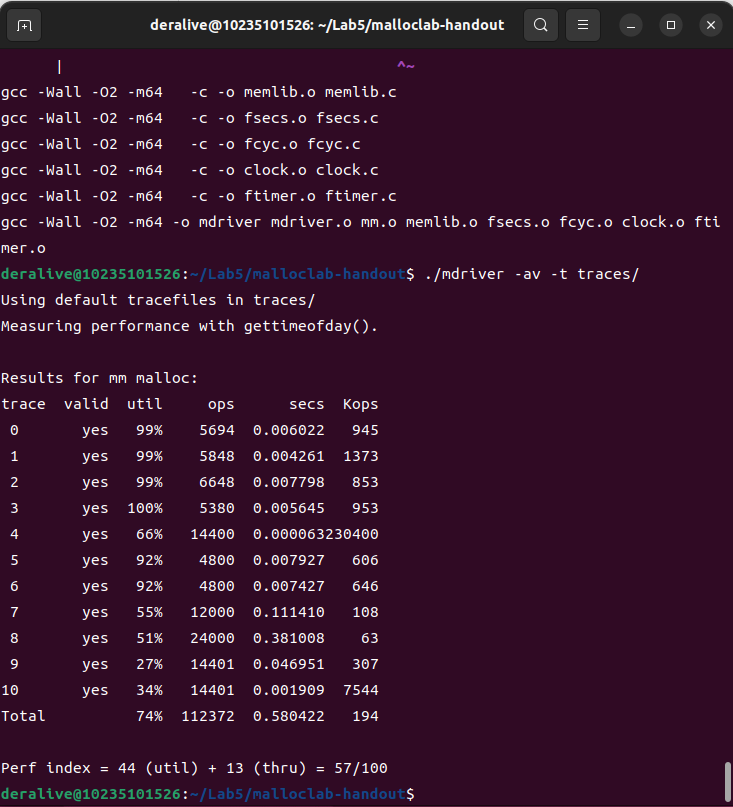
\includegraphics[width=0.5\textwidth]{Result.png}
    \caption{Result}
\end{figure}

可以看到,我们获得了$44$的$Util$分,$13$的$Thru$分,总分为$57$。

这个分数是一个看起来尚未及格的分数,我后续将考虑使用其他方法来优化。


% \section{Part B 实验内容}
% \subsection{简介}
按照官方文档的说明,需要在 trans.c 中写入一个优化的矩阵转置函数。
尽可能地降低不命中率。
使用命令:$./test-trans -M <rol> -N <col>$可以查看这一转置函数的不命中数。
生成的 trace.fi 文件还可以利用 PART A 写的缓存模拟器检查命中情况。

\begin{figure} [H]
    \centering
    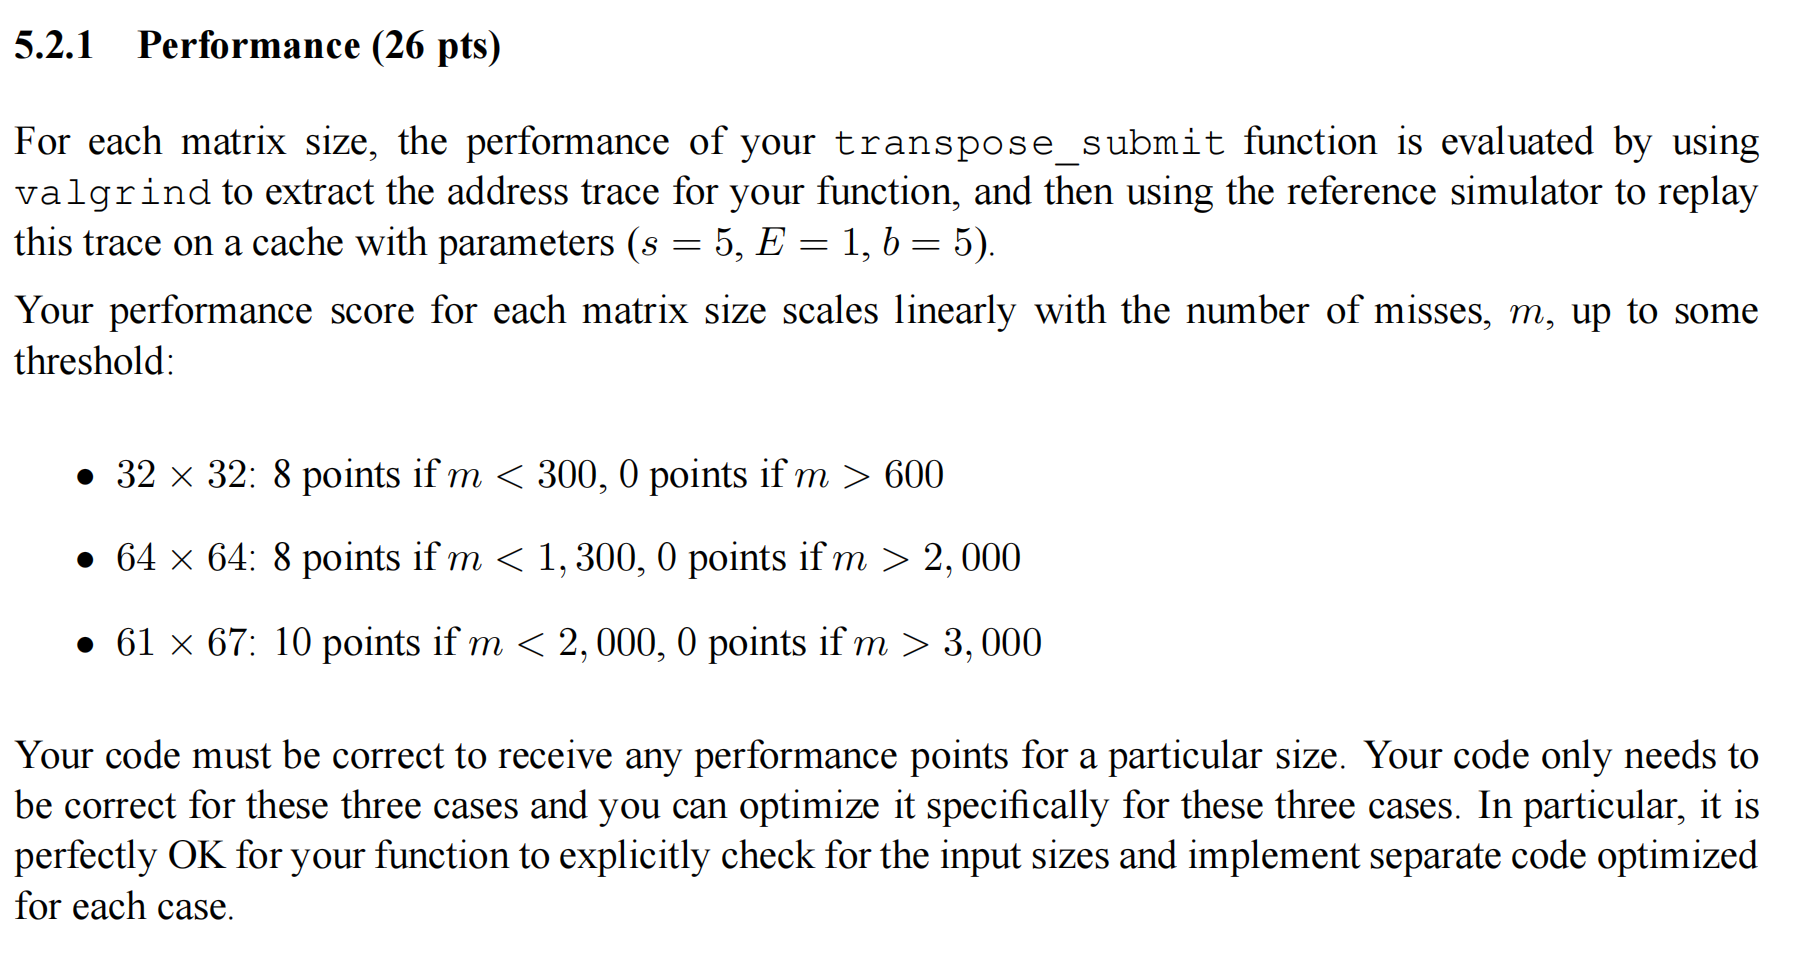
\includegraphics[width=0.52\textwidth]{PartBIntro.png}
    \caption{官方文档简介}
\end{figure}

\subsection{实验内容}
\subsubsection{Part B.1:$ 32 \times 32 $ 矩阵转置}
我们研究最简单的一个矩阵转置函数:
\begin{lstlisting}[language = C,title= Matrix Transpose]
int temp; A[32][32], B[32][32];
for (int i = 0; i < N; i++) {
    for (int j = 0; j < M; j++) {
        tmp = A[i][j];
        B[j][i] = temp;
    }
}
\end{lstlisting}

这是最简单的矩阵转置函数,它具有超过$ 1000 $ 的 $ Miss $数量。
我们可以通过优化这个函数来减少 $ Miss $ 数量。

所以可以利用矩阵分块的思想。每一行数组都可以被存入 4 个缓存行中,
一共有 32 个缓存行,所以每过 8 行就会出现一次和前面相同的组索引,
发生 $ miss $ 和 $ eviction $。所以考虑将 $ 32 \times 32 $ 的矩阵分成$ 16 $个 $8 \times 8 $的矩阵,
每一次都将一行的$ 8 $个 $ int $分别存储进 $t1 - t4$。
即,将矩阵划分成如下结构:

\begin{table}[h!]
    \centering
    \begin{tabular}{|c|c|c|c|}
        \hline
        1 & 2  & 3  & 4  \\
        \hline
        5 & 6  & 7  & 8  \\
        \hline
        9 & 10 & 11 & 12 \\
        \hline
    \end{tabular}
    \caption{Cache Struct (其中每一个小块都是 $ 8 \times 8 $)}
\end{table}

\begin{lstlisting}[language = C,title= Matrix Transpose]
/* 
* transpose_submit - This is the solution transpose function that you
*     will be graded on for Part B of the assignment. Do not change
*     the description string "Transpose submission", as the driver
*     searches for that string to identify the transpose function to
*     be graded. 
*/
char transpose_submit_desc[] = "Transpose submission";
void transpose_submit(int M, int N, int A[N][M], int B[M][N])
{
    if (N == 32 && M == 32)
    {
        int i, j, k;
        int t1, t2, t3, t4, t5, t6, t7, t8;
        for (i = 0; i < 32; i += 8)
        {
            for (j = 0; j < 32; j += 8)
            {
                for (k = 0; k < 8; k++)
                {
                    t1 = A[i + k][j];
                    t2 = A[i + k][j + 1];
                    t3 = A[i + k][j + 2];
                    t4 = A[i + k][j + 3];
                    t5 = A[i + k][j + 4];
                    t6 = A[i + k][j + 5];
                    t7 = A[i + k][j + 6];
                    t8 = A[i + k][j + 7];
                    B[j][i + k] = t1;
                    B[j + 1][i + k] = t2;
                    B[j + 2][i + k] = t3;
                    B[j + 3][i + k] = t4;
                    B[j + 4][i + k] = t5;
                    B[j + 5][i + k] = t6;
                    B[j + 6][i + k] = t7;
                    B[j + 7][i + k] = t8;
                }
            }
        }
    }
}
\end{lstlisting}

实验结果如下所示:
\begin{figure} [H]
    \centering
    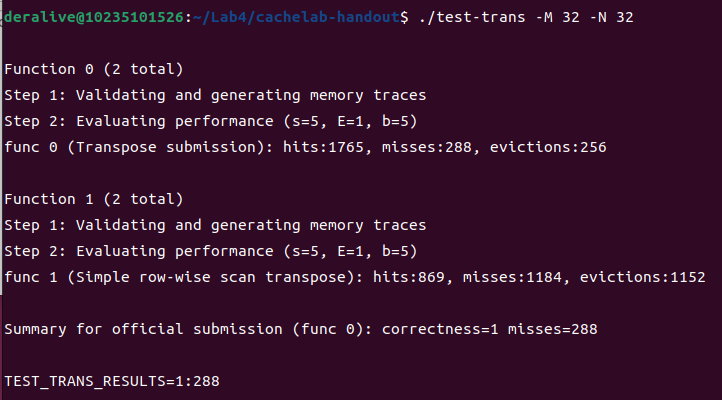
\includegraphics[width=0.52\textwidth]{PartB1.png}
    \caption{Part B.1 结果}
\end{figure}

\subsubsection{Part B.2:$ 64 \times 64 $ 矩阵转置}
大小变成了  $64 \times 64$ ,每过 $4$ 行就会出现一次冲突的情况。

所以可以先分成$ 8 \times 8 $ 的块,然后再把 $8 \times 8$ 的块分成 $4$ 个 $4 \times 4 $的块。

我们这里需要优化的不是程序运行的时间,而是cache的命中率。
具体是每一个$8 \times 8 $ 块中,分别移动$4 \times 4$ 的块,这样可以减少冲突。

\begin{itemize}
    \item 将 $ 8 \times 8  fence $分成 $ 4 \times 4 $ 的 fence, 再将角块分为 $ A、 B 、C、D$;
    \item 将$A $区的第一行缓存到$A' $和 $C'$ 的第一列
    \item 全部存到$ A' $和 $C'$ 后,再将C' 的第一列存到$ Temp1 \& Temp2 \& Temp3 \& Temp4 $变量当中
    \item 手动交换$C'$ 区 和 $B'$ 区的各个数值
\end{itemize}

\begin{figure} [H]
    \centering
    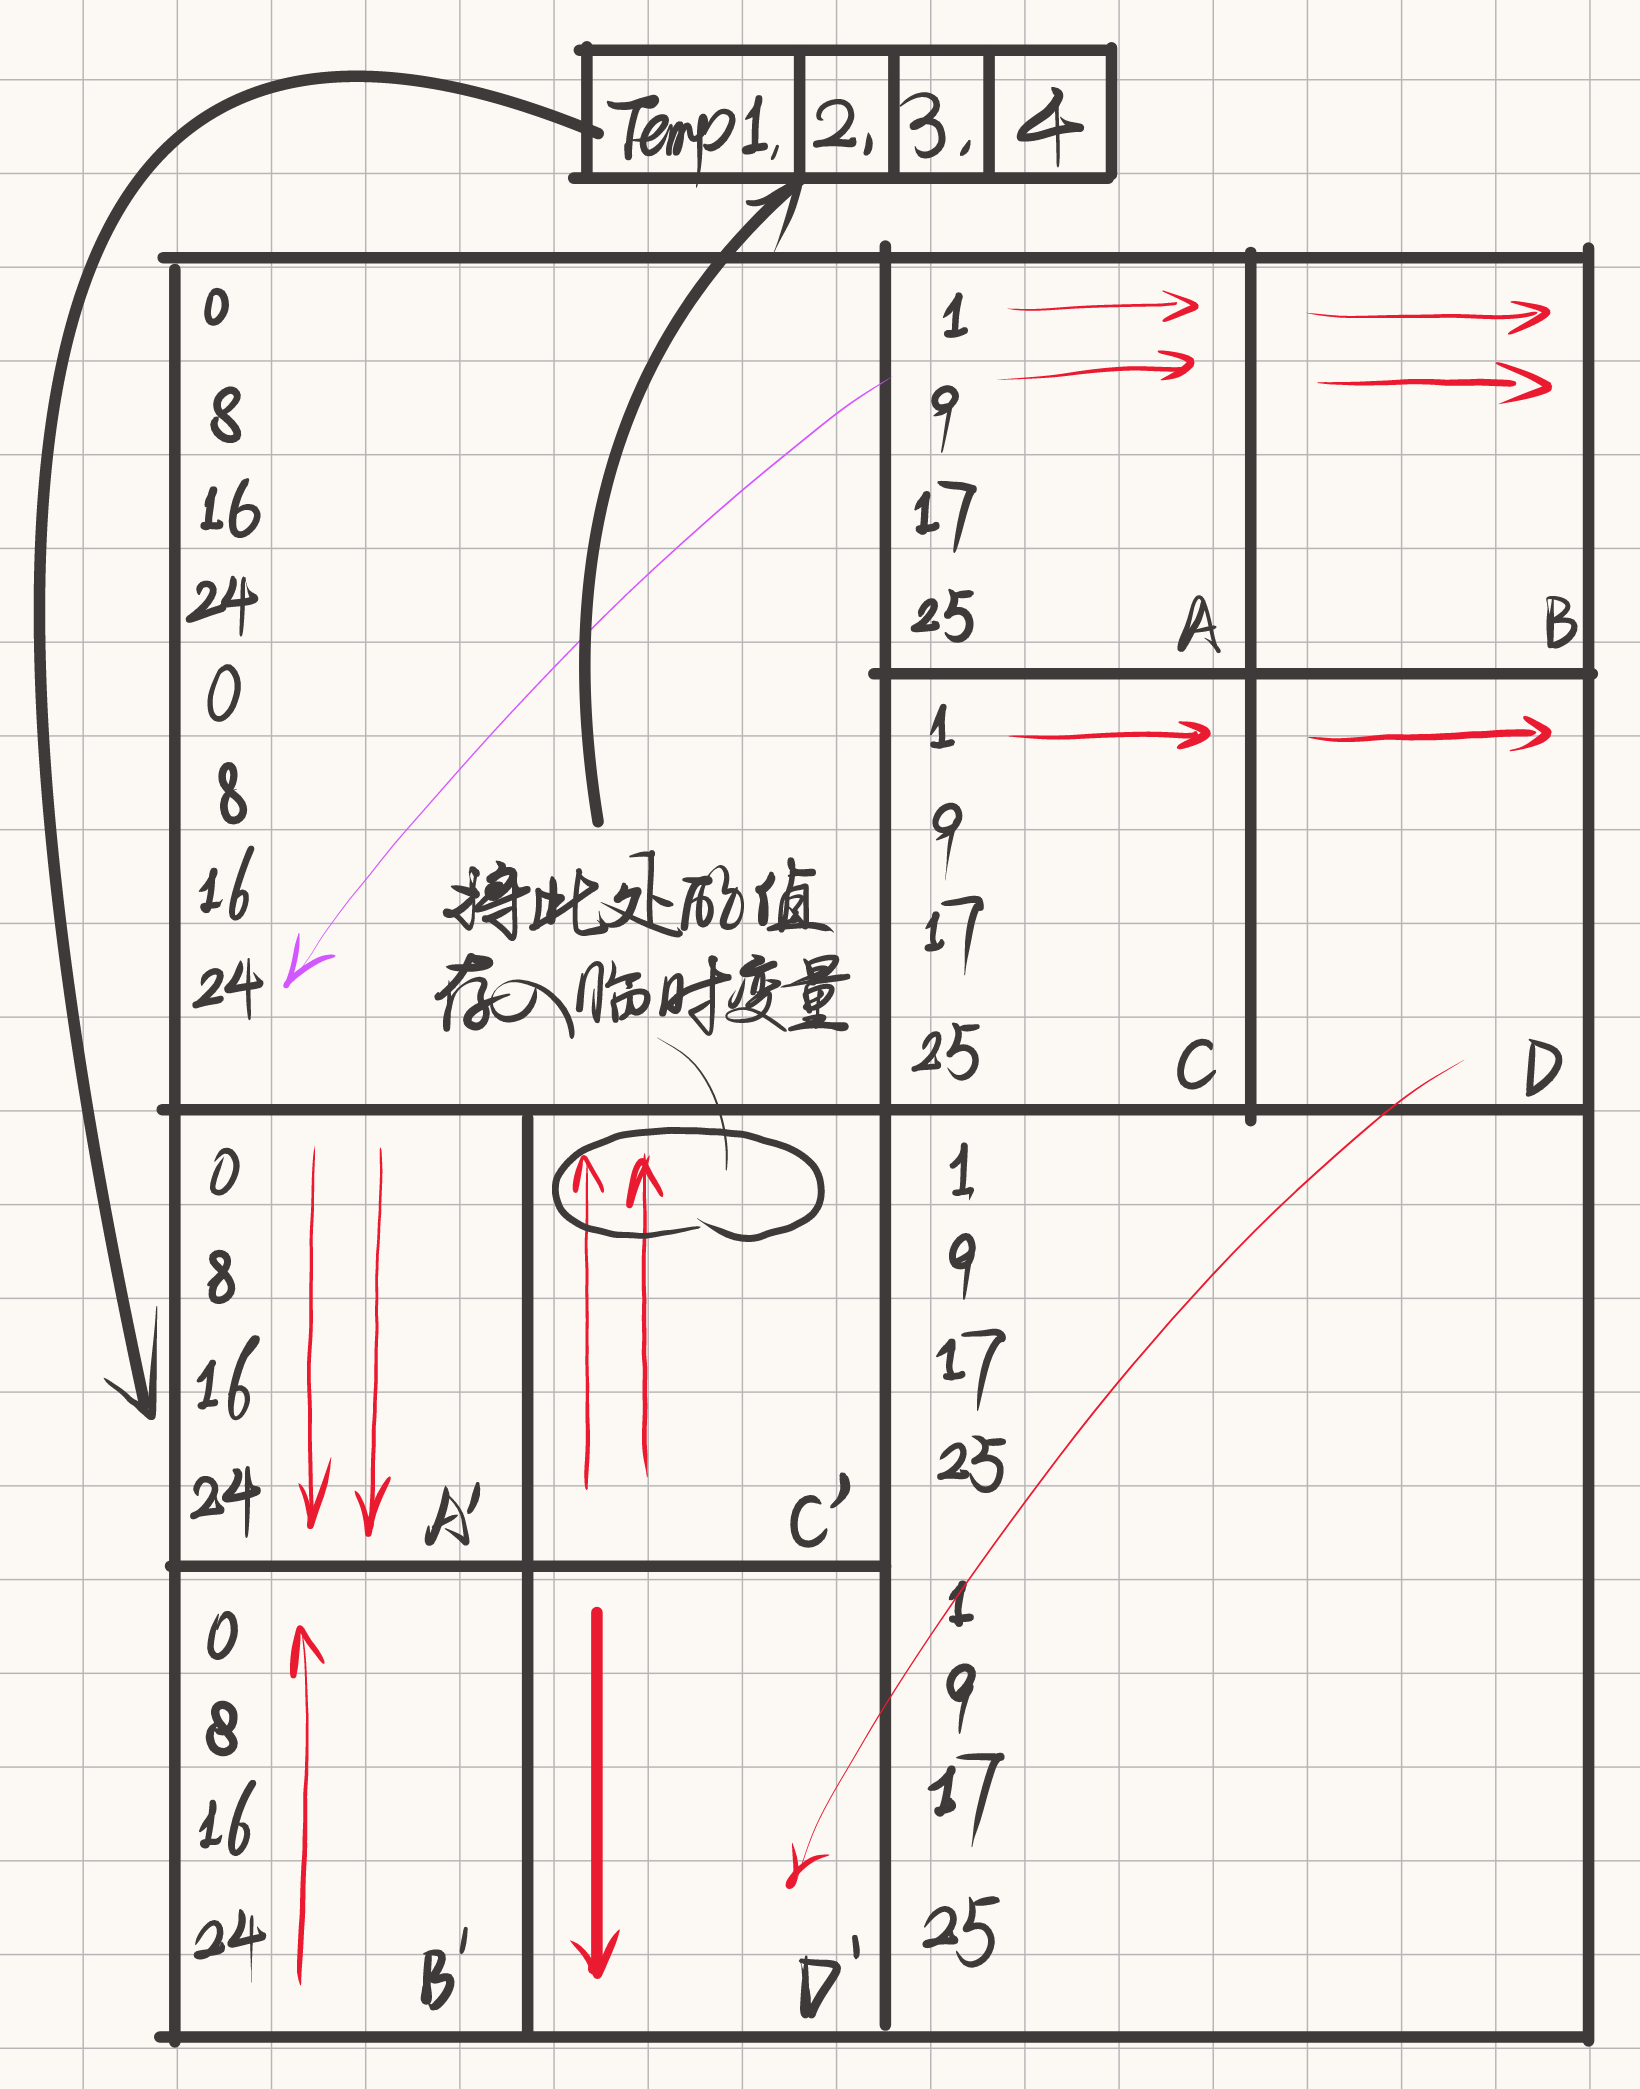
\includegraphics[width=0.38\textwidth]{Analy.png}
    \caption{Analysis Process}
\end{figure}


\begin{lstlisting}[language = C,title= Matrix Transpose]
else if (N == 64 && M == 64)
{
    int t0, t1, t2, t3, t4, t5, t6, t7;
    for (int i = 0; i < N; i += 8)
    {
        for (int j = 0; j < M; j += 8)
        {
            for (int k = i; k < i + 4; k++)
            {
                t0 = A[k][j];
                t1 = A[k][j + 1];
                t2 = A[k][j + 2];
                t3 = A[k][j + 3];
                t4 = A[k][j + 4];
                t5 = A[k][j + 5];
                t6 = A[k][j + 6];
                t7 = A[k][j + 7];
                B[j][k] = t0;
                B[j + 1][k] = t1;
                B[j + 2][k] = t2;
                B[j + 3][k] = t3;
                B[j + 0][k + 4] = t7;
                B[j + 1][k + 4] = t6;
                B[j + 2][k + 4] = t5;
                B[j + 3][k + 4] = t4;
            }
            for (int h = 0; h < 4; h++)
            {
                t0 = A[i + 4][j + 3 - h];
                t1 = A[i + 5][j + 3 - h];
                t2 = A[i + 6][j + 3 - h];
                t3 = A[i + 7][j + 3 - h];
                t4 = A[i + 4][j + 4 + h];
                t5 = A[i + 5][j + 4 + h];
                t6 = A[i + 6][j + 4 + h];
                t7 = A[i + 7][j + 4 + h];
                B[j + 4 + h][i + 0] = B[j + 3 - h][i + 4];
                B[j + 4 + h][i + 1] = B[j + 3 - h][i + 5];
                B[j + 4 + h][i + 2] = B[j + 3 - h][i + 6];
                B[j + 4 + h][i + 3] = B[j + 3 - h][i + 7];
                B[j + 3 - h][i + 4] = t0;
                B[j + 3 - h][i + 5] = t1;
                B[j + 3 - h][i + 6] = t2;
                B[j + 3 - h][i + 7] = t3;
                B[j + 4 + h][i + 4] = t4;
                B[j + 4 + h][i + 5] = t5;
                B[j + 4 + h][i + 6] = t6;
                B[j + 4 + h][i + 7] = t7;
            }
        }
    }
}
\end{lstlisting}

实验结果如下所示:

\begin{figure} [H]
    \centering
    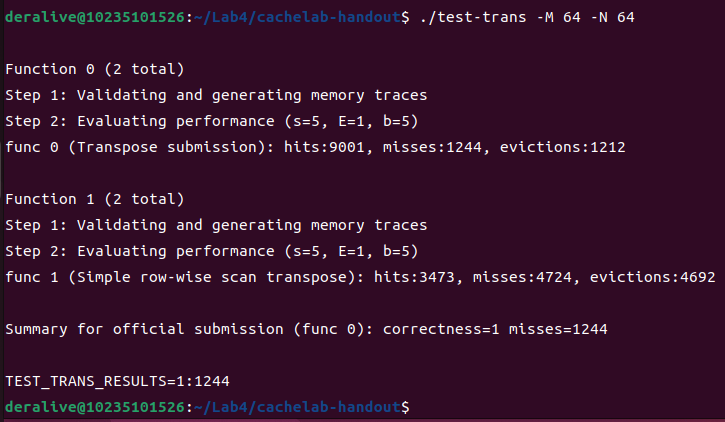
\includegraphics[width=0.52\textwidth]{PartB2.png}
    \caption{Part B.2 结果}
\end{figure}

\subsubsection{Part B.3:$ 61 \times 67 $ 矩阵转置}
这里的矩阵大小是 $61 \times 67$ ,这个矩阵的大小是一个奇数,所以不能被整除。
而且也不是 $ 8 $ 的倍数,所以在行与行之间没有特别明显的冲突不命中的关系。
可以尝试用分块矩阵的方式优化。经过尝试 $ 8 \times 8 $ 的分块和 $ 16 \times 16 $的分块后,
发现使用 $16 \times 16 $的分块方式可以将 $Miss$ 数降低到 $ 2000 $以下。

代码如下所示:
\begin{lstlisting}[language = C,title= Matrix Transpose]
else {
    int i, j, k, h;
    for (i = 0; i < N; i += 16) {
        for (j = 0; j < M; j += 16) {
            for (k = i; k < i + 16 && k < N; k++) {
                for (h = j; h < j + 16 && h < M; h++) {
                    B[h][k] = A[k][h];
                }
            }
        }
    }
}
\end{lstlisting}

实验结果如下所示:

\begin{figure} [H]
    \centering
    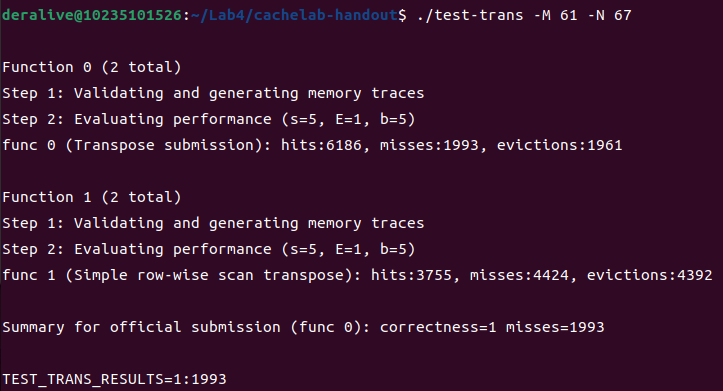
\includegraphics[width=0.52\textwidth]{PartF.png}
    \caption{Part B.3 结果}
\end{figure}







\section{实验总结}
通过这次实验,我学习了如何通过优化矩阵转置函数来提高缓存的命中率。
通过分块的方式,我们可以将不命中率降低到 $2000$ 以下。
这次实验让我更深入地了解了缓存的工作原理,也让我对缓存的优化有了更深的认识。
更重要的是,我学会了LateX,我会继续使用它来写实验报告。


\section{附录}
实验的源代码如下所示:
\begin{lstlisting} [language = C, title = {Appendix.c}]
    /* single word (4) or double word (8) alignment */
#define ALIGNMENT 8

#define WSIZE 4             // Word and header/footer size (bytes)
#define DSIZE 8             // Double word size (bytes)
#define CHUNKSIZE (1 << 12) // Extend heap by this amount (bytes)

#define MAX(x, y) ((x) > (y) ? (x) : (y)) // Maximum of two values

#define PACK(size, alloc) ((size) | (alloc)) // Pack a size and allocated bit into a word

#define GET(p) (*(unsigned int *)(p))              // Read a word at address p
#define PUT(p, val) (*(unsigned int *)(p) = (val)) // Write a word at address p
#define GET_SIZE(p) (GET(p) & ~0x7)                // Read the size and allocated fields from address p
#define GET_ALLOC(p) (GET(p) & 0x1)                // Read the allocated field from address p

// Given block ptr bp, compute address of its header and footer
#define HDRP(bp) ((char *)(bp) - WSIZE)
#define FTRP(bp) ((char *)(bp) + GET_SIZE(HDRP(bp)) - DSIZE)

// Given block ptr bp, compute address of next and previous blocks
#define NEXT_BLKP(bp) ((char *)(bp) + GET_SIZE(((char *)(bp) - WSIZE)))
#define PREV_BLKP(bp) ((char *)(bp) - GET_SIZE(((char *)(bp) - DSIZE)))

/* rounds up to the nearest multiple of ALIGNMENT */
#define ALIGN(size) (((size) + (ALIGNMENT - 1)) & ~0x7)

#define SIZE_T_SIZE (ALIGN(sizeof(size_t)))

/* 内部编程的函数原型 */
static void *extend_heap(size_t words);    // 扩展堆
static void *coalesce(void *bp);           // 合并空闲块
static void *find_fit(size_t size);        // 查找合适的空闲块
static void place(void *bp, size_t asize); // 分配空闲块

static char *heap_listp = 0; // 指向块首的指针

/*
 * mm_init - initialize the malloc package.
 */
int mm_init(void) {
    /* Create the initial empty heap */
    if ((heap_listp = mem_sbrk(4 * WSIZE)) == (void *) -1) // 申请4个字节
        return -1;
    PUT(heap_listp, 0);                            // Alignment padding
    PUT(heap_listp + (1 * WSIZE), PACK(DSIZE, 1)); // Prologue header
    PUT(heap_listp + (2 * WSIZE), PACK(DSIZE, 1)); // Prologue footer
    PUT(heap_listp + (3 * WSIZE), PACK(0, 1));     // Epilogue header
    heap_listp += (2 * WSIZE);                     // 指向序言块的头部

    /* Extend the empty heap with a free block of CHUNKSIZE bytes */
    if (extend_heap(CHUNKSIZE / WSIZE) == NULL) // 扩展堆
        return -1;                              // 扩展失败
    return 0;                                   // 成功
}

/*
 * mm_malloc - Allocate a block by incrementing the brk pointer.
 *     Always allocate a block whose size is a multiple of the alignment.
 */
void *mm_malloc(size_t size) {
    size_t asize;
    size_t extendsize;
    char *bp;
    if (size == 0)
        return NULL;
    if (size <= DSIZE) {
        asize = 2 * (DSIZE);
    } else {
        asize = (DSIZE) * ((size + (DSIZE) + (DSIZE - 1)) / (DSIZE));
    }
    if ((bp = find_fit(asize)) != NULL) {
        place(bp, asize);
        return bp;
    }
    extendsize = MAX(asize, CHUNKSIZE);
    if ((bp = extend_heap(extendsize / WSIZE)) == NULL) {
        return NULL;
    }
    place(bp, asize);
    return bp;
}

static void place(void *bp, size_t asize) {
    size_t csize = GET_SIZE(HDRP(bp));
    if ((csize - asize) >= (2 * DSIZE)) {
        PUT(HDRP(bp), PACK(asize, 1));
        PUT(FTRP(bp), PACK(asize, 1));
        bp = NEXT_BLKP(bp);
        PUT(HDRP(bp), PACK(csize - asize, 0));
        PUT(FTRP(bp), PACK(csize - asize, 0));
    } else {
        PUT(HDRP(bp), PACK(csize, 1));
        PUT(FTRP(bp), PACK(csize, 1));
    }
}

static void *coalesce(void *bp) {
    size_t prev_alloc = GET_ALLOC(FTRP(PREV_BLKP(bp)));
    size_t next_alloc = GET_ALLOC(HDRP(NEXT_BLKP(bp)));
    size_t size = GET_SIZE(HDRP(bp));
    if (prev_alloc && next_alloc) {
        return bp;
    } else if (prev_alloc && !next_alloc) {
        size += GET_SIZE(HDRP(NEXT_BLKP(bp)));
        PUT(HDRP(bp), PACK(size, 0));
        PUT(FTRP(bp), PACK(size, 0));
    } else if (!prev_alloc && next_alloc) {
        size += GET_SIZE(HDRP(PREV_BLKP(bp)));
        PUT(FTRP(bp), PACK(size, 0));
        PUT(HDRP(PREV_BLKP(bp)), PACK(size, 0));
        bp = PREV_BLKP(bp);
    } else {
        size += GET_SIZE(FTRP(NEXT_BLKP(bp))) + GET_SIZE(HDRP(PREV_BLKP(bp)));
        PUT(FTRP(NEXT_BLKP(bp)), PACK(size, 0));
        PUT(HDRP(PREV_BLKP(bp)), PACK(size, 0));
        bp = PREV_BLKP(bp);
    }
    return bp;
}

static void *extend_heap(size_t words) {
    char *bp;
    size_t size;
    size = (words % 2) ? (words + 1) * WSIZE : words * WSIZE;
    if ((long) (bp = mem_sbrk(size)) == (void *) -1)
        return NULL;
    PUT(HDRP(bp), PACK(size, 0));
    PUT(FTRP(bp), PACK(size, 0));
    PUT(HDRP(NEXT_BLKP(bp)), PACK(0, 1));
    return coalesce(bp);
}

static void *find_fit(size_t asize) {
    void *bp;
    for (bp = heap_listp; GET_SIZE(HDRP(bp)) > 0; bp = NEXT_BLKP(bp)) {
        if (!GET_ALLOC(HDRP(bp)) && (asize <= GET_SIZE(HDRP(bp)))) {
            return bp;
        }
    }
    return NULL;
}

/*
 * mm_free - Freeing a block does nothing.
 */
void mm_free(void *bp) {
    if (bp == 0)
        return;                       // 无效指针
    size_t size = GET_SIZE(HDRP(bp)); // 获取块大小
    PUT(HDRP(bp), PACK(size, 0));     // 标记为未分配
    PUT(FTRP(bp), PACK(size, 0));     // 标记为未分配
    coalesce(bp);                     // 合并空闲块
}

/*
 * mm_realloc - Implemented simply in terms of mm_malloc and mm_free
 */
void *mm_realloc(void *ptr, size_t size) {
    size_t oldsize;
    void *newptr;
    /* If size == 0 then this is just free, and we return NULL. */
    if (size == 0) {
        mm_free(ptr);
        return 0;
    }
    /* If oldptr is NULL, then this is just malloc. */
    if (ptr == NULL) {
        return mm_malloc(size);
    }
    newptr = mm_malloc(size);
    /* If realloc() fails the original block is left untouched  */
    if (!newptr) {
        return 0;
    }
    /* Copy the old data. */
    oldsize = GET_SIZE(HDRP(ptr));
    if (size < oldsize)
        oldsize = size;
    memcpy(newptr, ptr, oldsize);
    /* Free the old block. */
    mm_free(ptr);
    return newptr;
}
\end{lstlisting}


\end{document}